\documentclass[aspectratio=169]{beamer}
\usetheme{Bruno}
\usepackage{amsmath}
\usepackage{amssymb}
\usepackage{siunitx}
\usepackage{float}
\usepackage{tikz}
\def\checkmark{\tikz\fill[scale=0.4](0,.35) -- (.25,0) -- (1,.7) -- (.25,.15) -- cycle;} 
\usepackage{url}
\usepackage[siunitx,american,RPvoltages]{circuitikz}
\ctikzset{capacitors/scale=0.7}
\ctikzset{diodes/scale=0.7}
\usepackage{tabularx}
\newcolumntype{C}{>{\centering\arraybackslash}X}
\renewcommand\tabularxcolumn[1]{m{#1}}% for vertical centering text in X column
\usepackage{tabu}
\usepackage[spanish,es-tabla,activeacute]{babel}
\usepackage{babelbib}
\usepackage{booktabs}
\usepackage{pgfplots}
\usepackage{hyperref}
\hypersetup{colorlinks = true,
            linkcolor = black,
            urlcolor  = blue,
            citecolor = blue,
            anchorcolor = blue}
\usepgfplotslibrary{units, fillbetween} 
\pgfplotsset{compat=1.16}
\usepackage{bm}
\usetikzlibrary{arrows, arrows.meta, shapes, 3d, perspective, positioning,mindmap,trees,backgrounds}
\renewcommand{\sin}{\sen} %change from sin to sen
\usepackage{bohr}
\setbohr{distribution-method = quantum,insert-missing = true}
\usepackage{elements}
\usepackage{verbatim}
\usepackage[edges]{forest}
\usepackage{etoolbox}
\usepackage{schemata}
\usepackage{appendix}
\usepackage{listings}

\definecolor{color_mate}{RGB}{255,255,128}
\definecolor{color_plas}{RGB}{255,128,255}
\definecolor{color_text}{RGB}{128,255,255}
\definecolor{color_petr}{RGB}{255,192,192}
\definecolor{color_made}{RGB}{192,255,192}
\definecolor{color_meta}{RGB}{192,192,255}
\newcommand\diagram[2]{\schema{\schemabox{#1}}{\schemabox{#2}}}

\definecolor{codegreen}{rgb}{0,0.6,0}
\definecolor{codegray}{rgb}{0.5,0.5,0.5}
\definecolor{codepurple}{rgb}{0.58,0,0.82}
\definecolor{backcolour}{rgb}{0.95,0.95,0.92}

\lstdefinestyle{mystyle}{
    backgroundcolor=\color{backcolour},   
    commentstyle=\color{codegreen},
    keywordstyle=\color{magenta},
    numberstyle=\tiny\color{codegray},
    stringstyle=\color{codepurple},
    basicstyle=\ttfamily\footnotesize,
    breakatwhitespace=false,         
    breaklines=true,                 
    captionpos=b,                    
    keepspaces=true,                 
    numbers=left,                    
    numbersep=5pt,                  
    showspaces=false,                
    showstringspaces=false,
    showtabs=false,                  
    tabsize=2
}

\lstset{style=mystyle}
\title{Instrumentación I: \\ \emph{Introducción a la }\\ \emph{instrumentación industrial.} \\ \emph{Primera sesión}}
\author{
    Juan J. Rojas
}
\institute{Instituto Tecnológico de Costa Rica}
\date{\today}
\background{fig/background.jpg}
\begin{document}
\sisetup{unit-math-rm=\mathrm,math-rm=\mathrm} % change sinitx font
\sisetup{output-decimal-marker = {,}}
\maketitle

\newcommand{\blackandwhite}{white} %change this at the end

\begin{frame}{Señales}
    \begin{columns}[c, onlytextwidth]
        \begin{column}{0.6\textwidth}
        Una \textbf{señal} es la representación de una medición de una magnitud física que varía con una o más variables independientes y que porta información relevante.\\[8pt]
        Características: 
            \begin{itemize}
                \item Escalar o vectorial 
                \item Discreta o continua
                \item Determinista o aleatoria
            \end{itemize}    
        \end{column}
        \begin{column}{0.4\textwidth}
            \begin{center}
                \begin{tikzpicture}
                    \begin{axis}[
                        width= 0.9\linewidth,
                        height= 0.6\linewidth,
                        domain=0:4*pi,
                        samples=100,
                        ymin=-1.2, ymax=1.2,
                        xmin=0, xmax=4*pi+0.5,
                        axis x line=center,
                        axis y line=left,
                        ytick={\empty},
                        yticklabels={\empty},
                        xtick={\empty},
                        xticklabels={\empty},
                        %xtick={pi,2*pi,3*pi,4*pi},
                        %xticklabels={$\pi$,$2\pi$,$3\pi$,$4\pi$},
                        xlabel=$t$, % Set the labels
                        ylabel=$f(t)$,
                        x unit=, 
                        y unit=,
                        axis lines=center,
                        x label style={anchor=west},
                        y label style={anchor=south},
                        ]
                        \addplot[color=blue,mark=none,thick] {sin(deg(x))}
                    	;
                    \end{axis}
                    \begin{axis}[
                        yshift=-3cm,
                        width= 0.9\linewidth,
                        height= 0.6\linewidth,
                        domain=0:4*pi,
                        samples=100,
                        ymin=-1.2, ymax=1.2,
                        xmin=0, xmax=4*pi+0.5,
                        axis x line=center,
                        axis y line=left,
                        ytick={\empty},
                        yticklabels={\empty},
                        xtick={\empty},
                        xticklabels={\empty},
                        %xtick={pi,2*pi,3*pi,4*pi},
                        %xticklabels={$\pi$,$2\pi$,$3\pi$,$4\pi$},
                        xlabel=$p$, % Set the labels
                        ylabel=$f(p)$,
                        x unit=, 
                        y unit=,
                        axis lines=center,
                        x label style={anchor=west},
                        y label style={anchor=south},
                        ]
                        \addplot[color=red,mark=none,thick] {rand}
                    	;
                    \end{axis}
                \draw[\blackandwhite] (-0.5,-3.2) rectangle (4,2.5);
                \end{tikzpicture}
            \end{center}
        \end{column}
    \end{columns}
\end{frame}

\begin{frame}{Estímulos}
Magnitud física, del entorno o del sistema en estudio, que actúa sobre un sensor y que puede ser medida para generar una señal.\\[8pt]
Algunos ejemplos de estímulos: 
    \begin{itemize}
        \item Aceleración 
        \item Intensidad de radiación
        \item Temperatura
        \item Concentración de un componente químico
    \end{itemize}    
\end{frame}

\begin{frame}{Sistemas}
    \begin{columns}[c, onlytextwidth]
        \begin{column}{0.4\textwidth}
        Un sistema es una construcción o colección de diferentes elementos que juntos producen resultados que no pueden obtenerse con los elementos por separado\cite{INCOSE}.\\[8pt]
        Un sistema es un objeto o conjunto de objetos cuyas propiedades queremos estudiar\cite{modelica}.
        \end{column}
        \begin{column}{0.6\textwidth}
            \begin{center}
               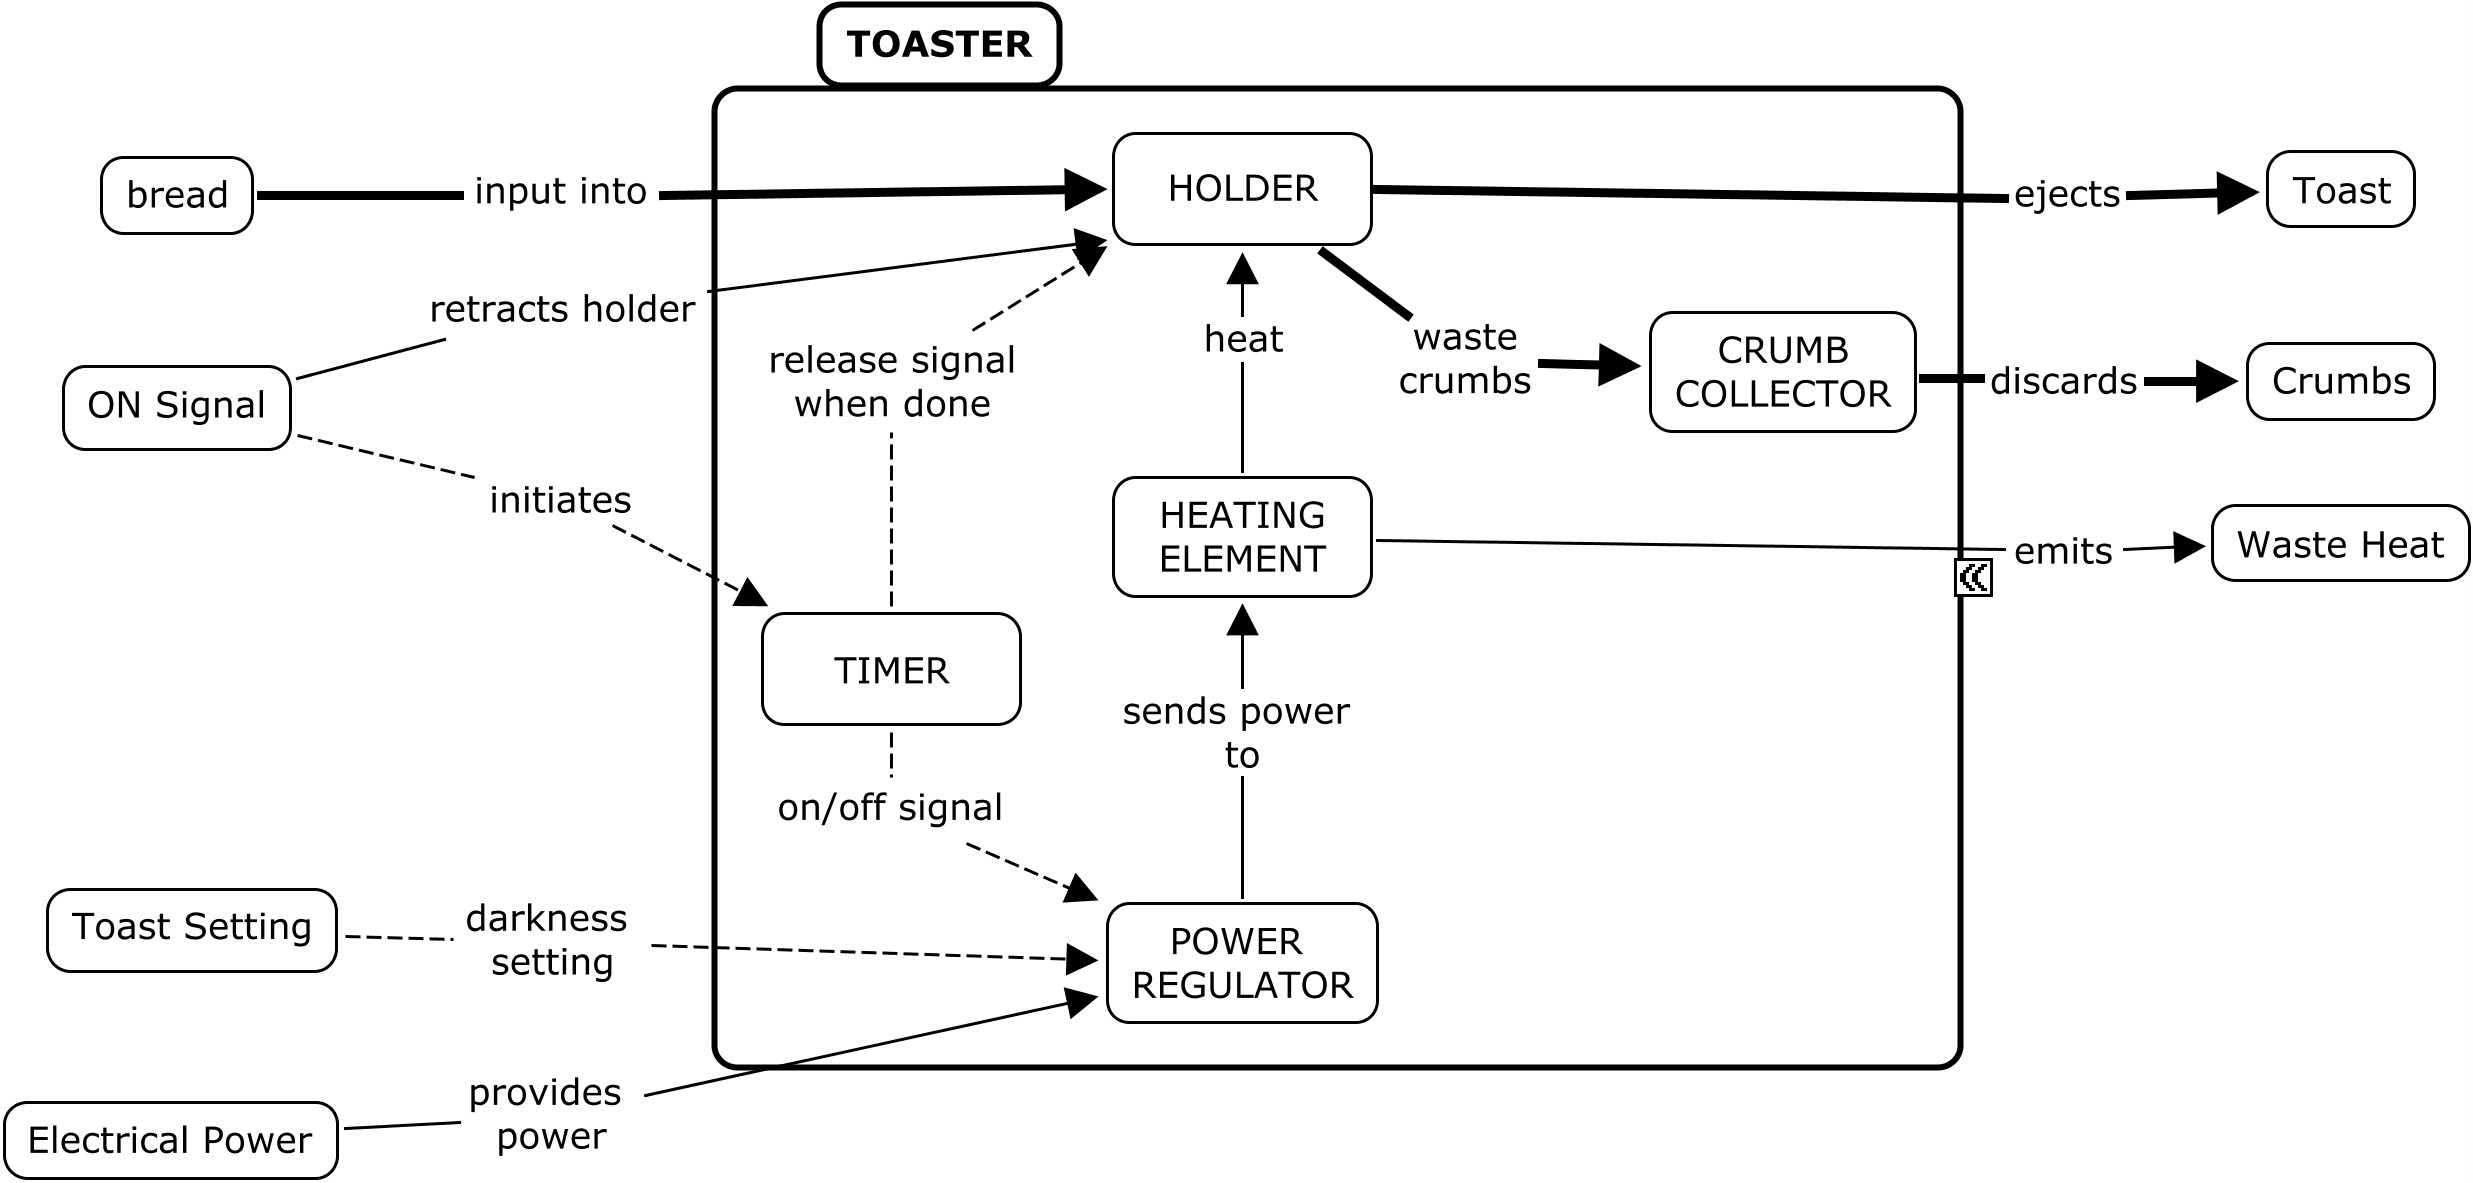
\includegraphics[width=\textwidth]{fig/tostadora.jpg}\\
               \tiny{Tomado de \href{https://deseng.ryerson.ca/dokuwiki/_detail/design:toasterarchitecture.jpg?id=design\%3Asystem_diagram}{aquí}}
            \end{center}
        \end{column}
    \end{columns}
\end{frame}

\begin{frame}{Señales de entrada y salida}
    \begin{columns}[c, onlytextwidth]
        \begin{column}{0.4\textwidth}
             \begin{itemize}
                \item Entradas: son las variables que afectan el comportamiento del sistema
                \item Salidas: son las variables que son definidas por el sistema
             \end{itemize}
        \end{column}
        \begin{column}{0.6\textwidth}
            \begin{center}
               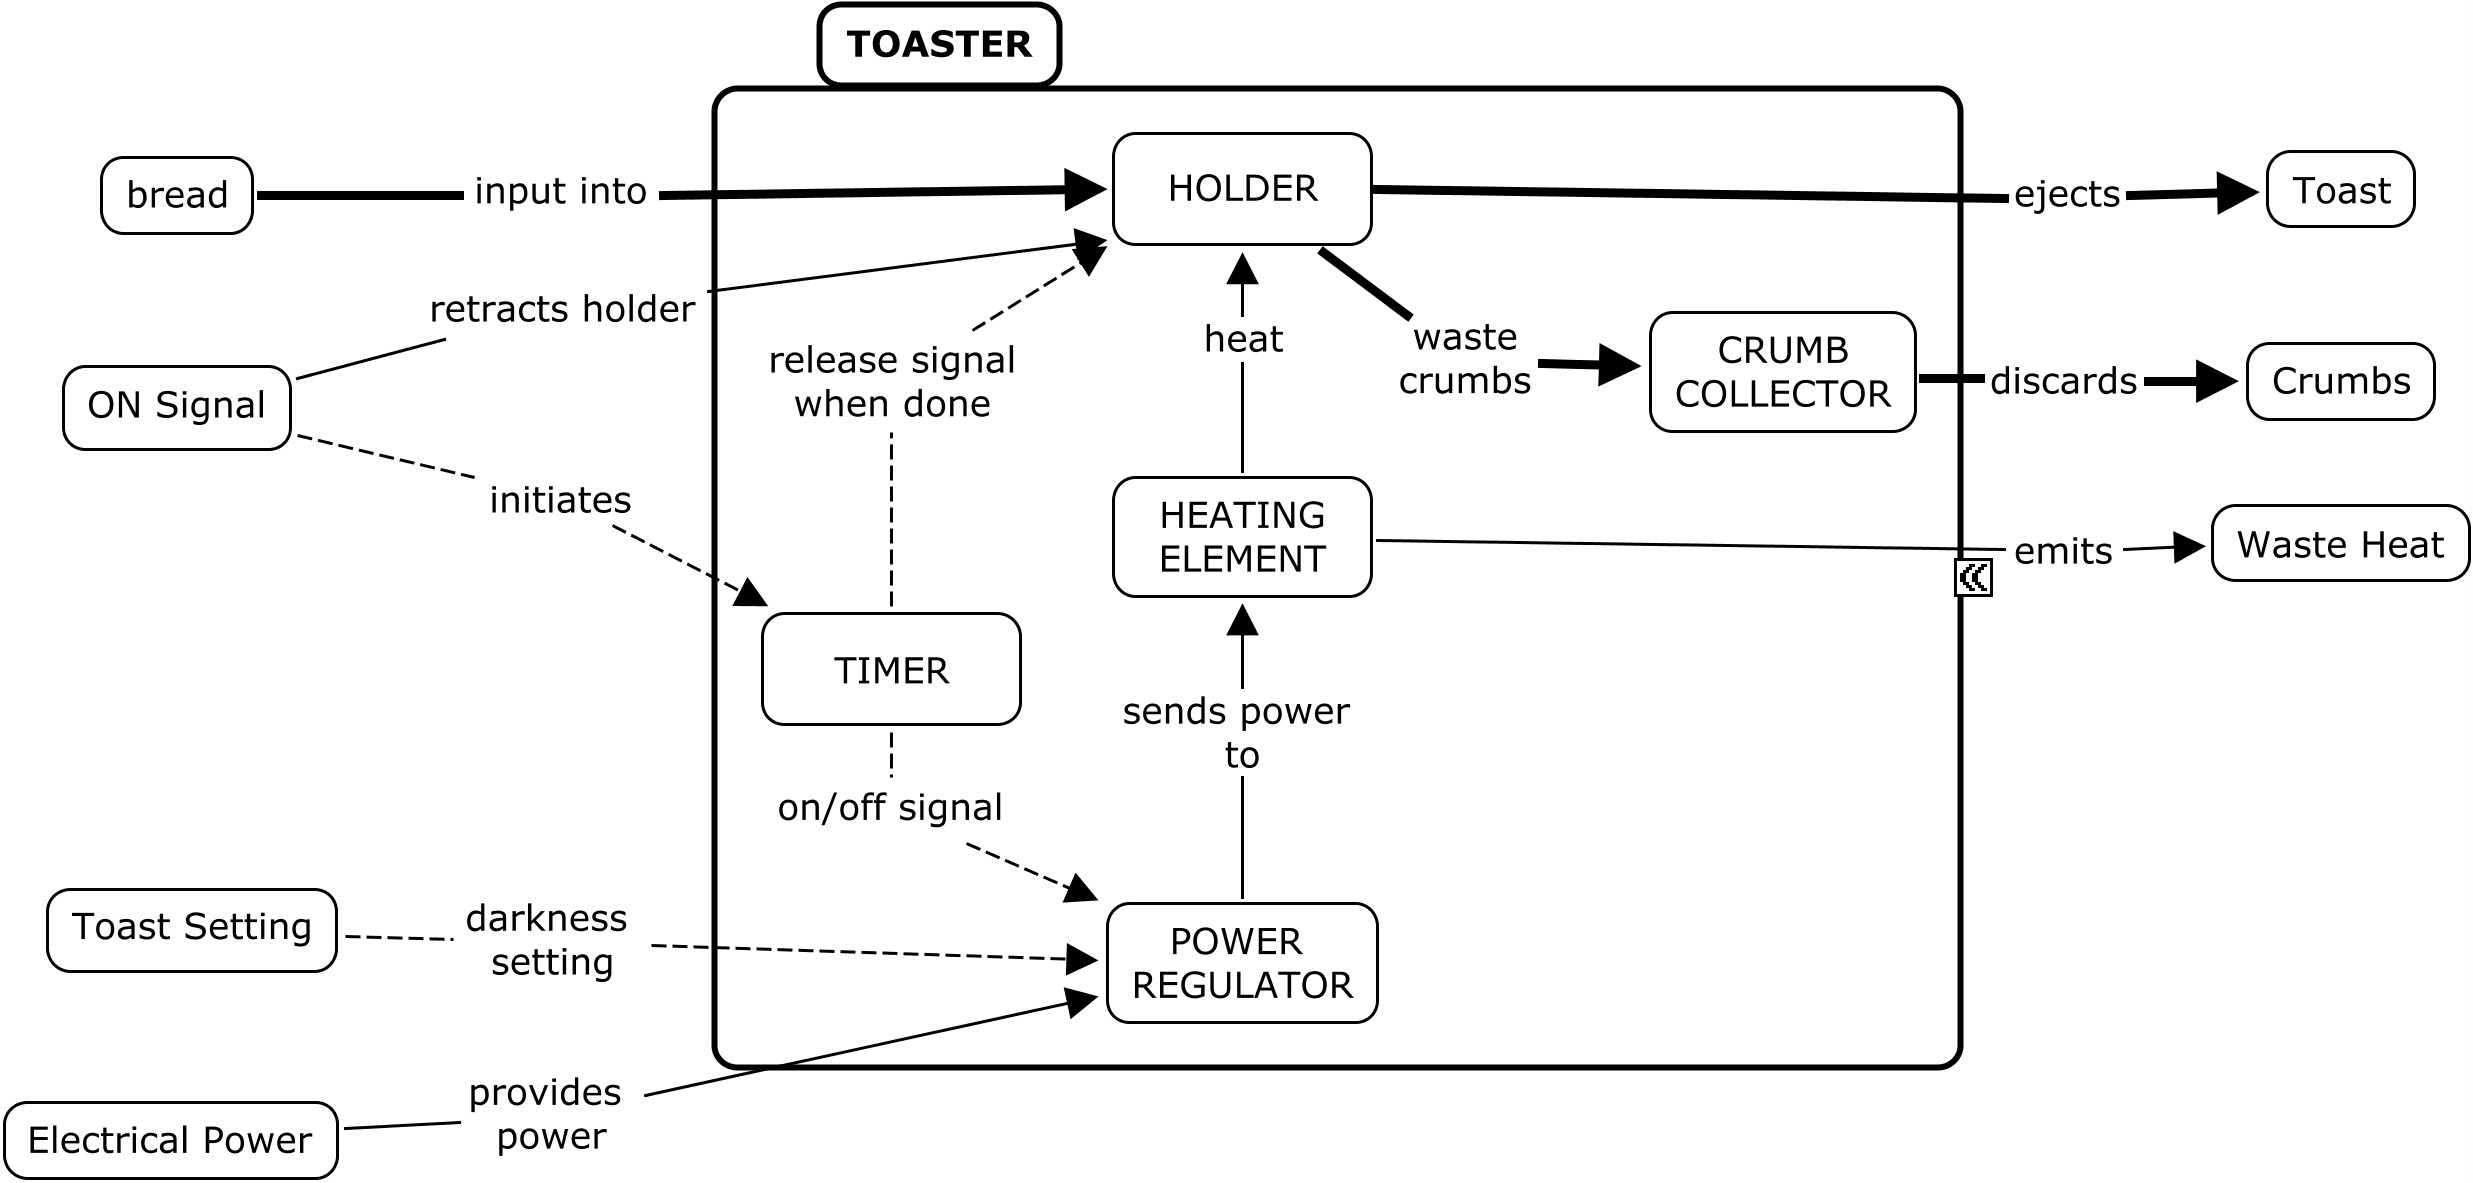
\includegraphics[width=\textwidth]{fig/tostadora.jpg}\\
               \tiny{Tomado de \href{https://deseng.ryerson.ca/dokuwiki/_detail/design:toasterarchitecture.jpg?id=design\%3Asystem_diagram}{aquí}}
            \end{center}
        \end{column}
    \end{columns}
\end{frame}

\begin{frame}{Modelos y simulaciones}
    \begin{columns}[c, onlytextwidth]
        \begin{column}{0.5\textwidth}
        Un modelo es una abstracción matemática de un sistema.\\[8pt]
        \begin{itemize}
            \item Se modela el sistema en base a ecuaciones
            \item Es una simplificación del sistema real
            \item Solo es valido en ciertas condiciones y/o rangos
        \end{itemize}
        Una simulación es un experimento que se realiza en el modelo de un sistema.
        
        \end{column}
        \begin{column}{0.5\textwidth}
            \begin{center}
                \begin{circuitikz}
                    \draw 
                    (0,0)
                        to[cV, l=$OCV(z)$]
                    (0,3)
                        to[R, l=$R_0$,i=$i(t)$,-o]
                    (3,3)
                        to[open,v^=$v(t)$]
                    (3,0)
                        to[short,o-]
                    (0,0)
                    ;
                \end{circuitikz}\\[8pt]
                \footnotesize{Modelo Rint de una celda electroquímica}
            \end{center}
        \end{column}
    \end{columns}
\end{frame}

\begin{frame}{Transductores, sensores y actuadores}
    \begin{columns}[c, onlytextwidth]
        \begin{column}{0.6\textwidth}
        Para los efectos de este curso...\\[8pt]
        \begin{itemize}
            \item \textbf{Transductor:} dispositivo que convierte una señal de un tipo de energía a una señal correspondiente pero con un tipo de energía diferente.
            \item \textbf{Sensor:} transductor que convierte una señal física a un señal eléctrica
            \item \textbf{Actuador:} transductor que convierte una señal eléctrica a un señal física
        \end{itemize}
        \end{column}
        \begin{column}{0.4\textwidth}
            \begin{center}
               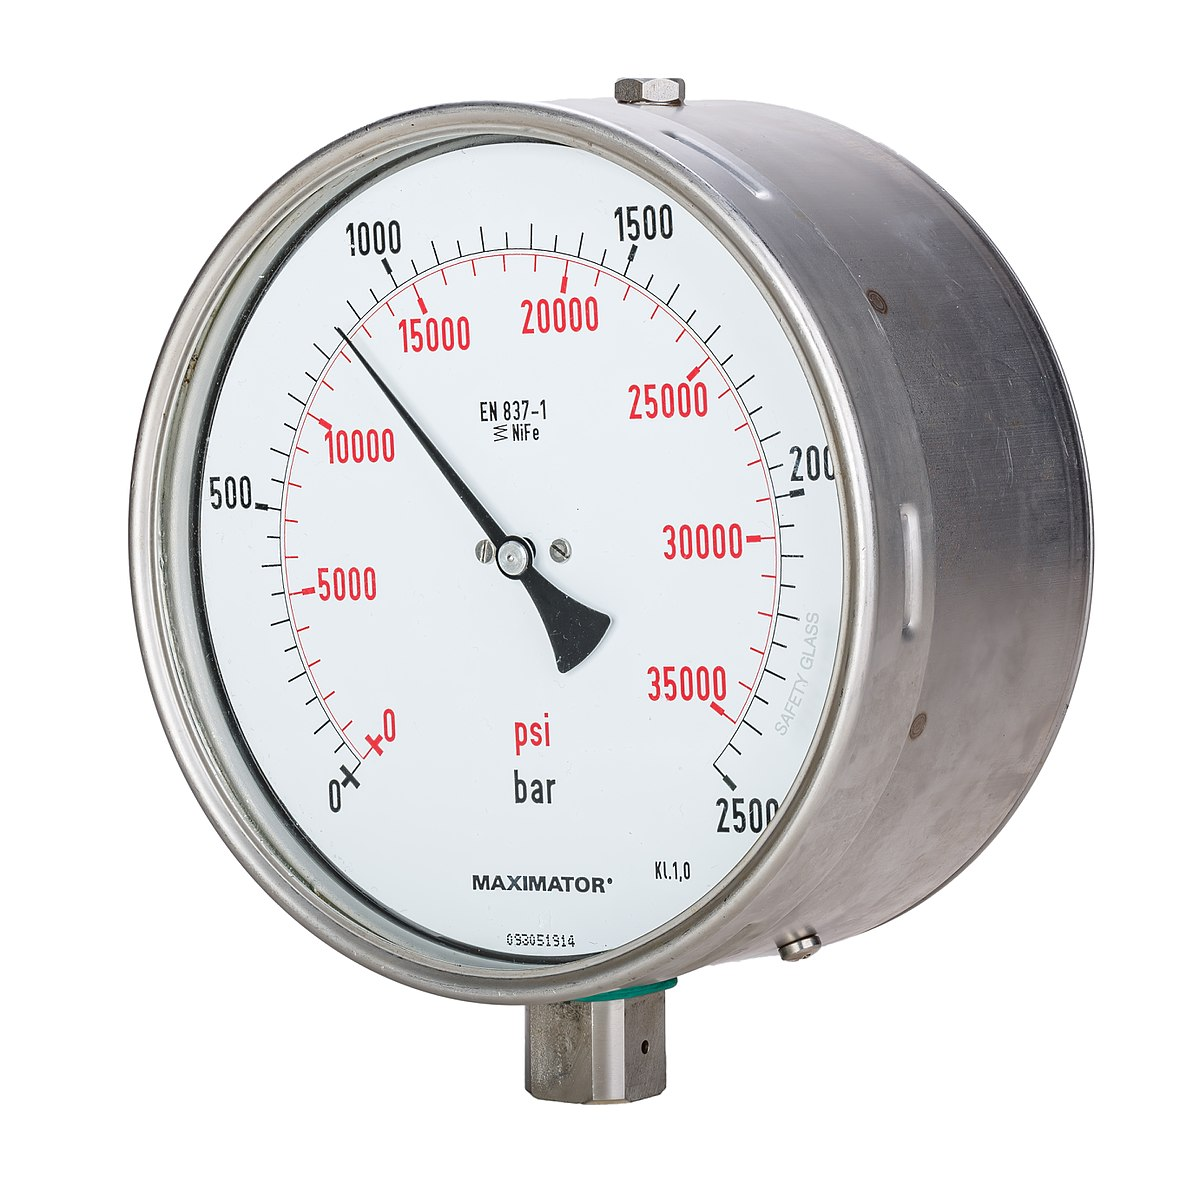
\includegraphics[width=0.8\textwidth]{fig/bourdon.jpg}\\
               \tiny{Tomado de \href{https://upload.wikimedia.org/wikipedia/commons/thumb/7/74/MAXIMATOR-High-Pressure-Manometer-01a.jpg/1200px-MAXIMATOR-High-Pressure-Manometer-01a.jpg}{aquí}}
            \end{center}
        \end{column}
    \end{columns}
\end{frame}

\begin{frame}{Sensores directos y complejos}
    \begin{columns}[c, onlytextwidth]
        \begin{column}{0.5\textwidth}
        Sensor directo
            \begin{tikzpicture}
                \node[draw,minimum width=2cm,minimum height=1.2cm](sensor) {sensor};
                \draw[>=latex, thick, ->](sensor) --++ (-3,0) -- (sensor);
                \node[left=1,above] at (sensor.west){\small estímulo};
                \draw[>=latex, thick, ->](sensor) -- (sensor) --++ (3,0);
                \node[right=1,above] at (sensor.east){\small señal};
                \node[right=1,below] at (sensor.east){\small eléctrica};
                \draw[\blackandwhite] (-3,-1.5) rectangle (3,3);
            \end{tikzpicture}
        \end{column}
        \begin{column}{0.5\textwidth}
        Sensor complejo
            \begin{tikzpicture}
            \node[draw,minimum width=1cm,minimum height=1cm](s1) {trans};
            \draw[>=latex, thick, ->](s1) --++ (-2,0) -- (s1);
            \node[left=0.75,above] at (s1.west){\small estímulo};
            \node[draw,minimum width=1cm,minimum height=1cm,right of=s1,node distance=2cm](s2) {sens};
            \draw[>=latex, thick, ->](s2) -- (s2) --++ (2,0);
            \node[right=0.75,above] at (s2.east){\small señal};
            \node[right=0.75,below] at (s2.east){\small eléctrica};
            \draw[>=latex, thick, ->](s1) -- (s2);
            \draw[\blackandwhite] (-2,-1.5) rectangle (4,3);
            \draw[black, dashed] (0.75,-1) rectangle (4,1.5)node[midway,above=0.7]{\small sensor directo};
            \end{tikzpicture}
        \end{column}
    \end{columns}
\end{frame}

\begin{frame}{Sensores pasivos y activos}
    \begin{columns}[c, onlytextwidth]
        \begin{column}{0.5\textwidth}
        Sensor pasivo
            \begin{tikzpicture}
                \node[draw,minimum width=2cm,minimum height=1.2cm](sensor) {sensor};
                \draw[>=latex, thick, ->](sensor) --++ (-3,0) -- (sensor);
                \node[left=1,above] at (sensor.west){\small estímulo};
                \draw[>=latex, thick, ->](sensor) -- (sensor) --++ (3,0);
                \node[right=1,above] at (sensor.east){\small señal};
                \node[right=1,below] at (sensor.east){\small eléctrica};
                \draw[\blackandwhite] (-3,-1.5) rectangle (3,3);
            \end{tikzpicture}
        \end{column}
        \begin{column}{0.5\textwidth}
        Sensor activo
            \begin{tikzpicture}
                \node[draw,minimum width=2cm,minimum height=1.2cm](sensor) {sensor};
                \draw[>=latex, thick, ->](sensor) --++ (-3,0) -- (sensor);
                \node[left=1,above] at (sensor.west){\small estímulo};
                \draw[>=latex, thick, ->](sensor) -- (sensor) --++ (3,0);
                \node[right=1,above] at (sensor.east){\small señal};
                \node[right=1,below] at (sensor.east){\small eléctrica};
                \draw[>=latex, thick, ->](sensor) --++ (0,+2) -- (sensor);
                \node[above=1.5] at (sensor.north){\small excitación};
                \draw[\blackandwhite] (-3,-1.5) rectangle (3,3);
            \end{tikzpicture}
        \end{column}
    \end{columns}
\end{frame}

\begin{frame}{Referencias}

\bibliographystyle{ieeetr}
\footnotesize
\bibliography{comunes/referencias}

\end{frame}

\end{document}